% KCC 2026 포스터 논문 (심사용 - 익명)
% Compile with XeLaTeX (Overleaf: Menu → Compiler → XeLaTeX)

\documentclass[a4paper,10pt]{article}

% --- 페이지 여백 (KCC 규정: 위 30mm, 아래 20mm, 좌/우 10mm) ---
\usepackage[a4paper,top=30mm,bottom=20mm,left=10mm,right=10mm]{geometry}

% --- 한글 ---
\usepackage{kotex}

% --- 기타 패키지 ---
\usepackage{multicol}
\usepackage{graphicx}
\usepackage{booktabs}
\usepackage{amsmath, amssymb}
\usepackage{url}
\usepackage{caption}
\usepackage{float}

% 캡션 설정
\captionsetup{font=small, labelfont=bf, skip=4pt}

% KCC 규정: 표는 "표 N", 그림은 "그림 N"
\renewcommand{\tablename}{표}
\renewcommand{\figurename}{그림}

% 문단 들여쓰기
\setlength{\parindent}{1em}
\setlength{\parskip}{0.2em}

% 단 사이 간격
\setlength{\columnsep}{6mm}

% 페이지 번호 제거 (KCC)
\pagestyle{empty}

\begin{document}

% =========================================================
% 1단 영역: 제목, 영문제목, 요약
% =========================================================
\begin{center}
{\Large\bfseries LoRA의 Anchor-Freedom 분업: SVD 초기화 전략의 학습 용량 정량 분석\par}
\vspace{0.5em}
{\large Anchor-Freedom Decomposition in LoRA: A Quantitative Analysis of SVD-based Initialization Strategies\par}
\vspace{1em}
% 익명 심사용: 저자/소속/이메일 미기재
\end{center}

\begin{center}
\begin{minipage}{0.92\textwidth}
\noindent\textbf{요\ \ 약}\\[0.3em]
\small
LoRA(Low-Rank Adaptation)의 두 행렬 $A$와 $B$의 초기화 방식에 따라 학습 동학과 성능이 크게 달라짐이 보고되어 왔으나 그 원리에 대한 통일된 이해는 부족하다.
본 연구는 LoRA의 두 행렬이 \textbf{anchor}(사전학습 가중치 $W$의 구조적 사전정보 제공)와 \textbf{freedom}(태스크 종속적 잔차 학습)으로 분업되어야 한다는 프레임워크를 제안하고, 학습된 $\Delta W$를 $W$로 정규화한 $W_{\text{rel}}$ 지표로 여섯 가지 초기화 전략을 정량 비교한다.
Llama-3.2-3B를 GSM8K와 HumanEval에서 미세조정한 결과, (1) PiSSA는 $A,B$ 모두 SVD로 강하게 anchor되어 $W_{\text{rel}}$이 1.34\%에 그치는 over-anchored 상태로 A-only SVD(2.39\%) 대비 학습 용량이 56\% 수준이며, (2) LoRA-FA의 무작위 $A$ 동결은 적절한 anchor를 제공하지 못해 다른 SVD 기반 기법 대비 GSM8K $-13.85$\%p, HumanEval $-4.06$\%p로 약세를 보인다.
(3) A-only / B-only SVD는 한쪽 anchor + 한쪽 freedom 분업이 작동하여 PiSSA를 두 태스크 모두에서 능가하며(HumanEval $+1.42$\%p), (4) 본 프레임워크의 최소 구현인 Frozen-A는 학습 파라미터를 49\% 감소시키면서도 표준 LoRA 대비 GSM8K $+3.54$\%p, HumanEval $+1.62$\%p 향상을 달성하며 PiSSA와 동등한 성능을 절반 용량으로 확보한다.
\end{minipage}
\end{center}
\vspace{1.5em}

% =========================================================
% 2단 영역: 본문
% =========================================================
\begin{multicols}{2}

\section*{1. 서 론}

거대 언어 모델(LLM)의 미세조정에서 파라미터 효율적 미세조정(PEFT)이 표준이 되었으며, 그 중 LoRA[1]는 사전 학습 가중치 $W$에 저랭크 갱신 $\Delta W = (\alpha/r) B A$를 더하는 방식으로 사실상 표준으로 자리잡았다. 여기서 $A \in \mathbb{R}^{r \times d_{in}}$, $B \in \mathbb{R}^{d_{out} \times r}$이며, 표준 구현은 $A$를 Kaiming 균등분포, $B$를 0으로 초기화한다.

LoRA의 초기화 전략을 변형한 다양한 후속 연구가 제안되어 왔다. PiSSA[2]는 $A,B$를 $W$의 SVD 상위 $r$개 성분으로 초기화하고, LoRA-FA[3]는 무작위 $A$를 동결하여 $B$만 학습하며, VeRA[4]는 모든 층의 $A,B$를 공유 동결하고 작은 스케일 벡터만 학습한다. 그러나 이러한 변형들이 \textit{왜} 서로 다른 결과를 내는지에 대한 통일된 메커니즘 설명은 부족하며, 각 기법이 개별 비교 실험 결과로만 비교되고 있다.

본 연구는 LoRA의 두 행렬이 \textbf{anchor와 freedom으로 분업되어야 한다}는 프레임워크를 제안한다. Anchor는 $W$의 구조적 사전정보를 제공하는 역할이며, freedom은 태스크 종속적 잔차를 학습할 용량을 담당한다. 한쪽이 강하게 anchor되면 다른 쪽이 freedom을 담당해야 하며, 양쪽 모두 강하게 anchor되면(PiSSA) 학습 용량이 제한된다. Anchor가 잘못된 방향이면(LoRA-FA의 무작위 $A$) 학습이 비효율적이다.

이 프레임워크를 정량 검증하기 위해 학습된 $\Delta W$의 크기를 $W$로 정규화한 $W_{\text{rel}} = \|\Delta W\|_F / \|W_{\text{pre}}\|_F$ 지표를 도입한다. Llama-3.2-3B에서 6가지 초기화 전략을 비교한 결과 다음을 확인하였다. (1) PiSSA는 $W_{\text{rel}}=1.34\%$로 다른 SVD 기반 기법 대비 학습 용량이 56\% 수준에 그치는 over-anchored 상태이고, (2) LoRA-FA(무작위 $A$ 동결)는 잘못된 anchor로 GSM8K에서 다른 SVD 기법 대비 $-13.85$\%p 약세이며, (3) A-only SVD와 B-only SVD는 한쪽 anchor + 한쪽 freedom 분업으로 PiSSA를 두 태스크 모두에서 능가하고, (4) 본 프레임워크의 최소 구현인 \textbf{Frozen-A}($A$=SVD anchor 동결 + $B$만 학습)는 학습 파라미터 49\% 감소에도 표준 LoRA 대비 GSM8K $+3.54$\%p, HumanEval $+1.62$\%p 향상을 달성한다.

\section*{2. 관련 연구}

LoRA[1]는 갱신을 저랭크 분해로 매개변수화하여 모델 파라미터의 0.1\% 미만의 추가 파라미터로 전체 미세조정에 근접한 성능을 달성한다. PiSSA[2]는 $W = U \Sigma V^\top$의 SVD 결과 중 상위 $r$개로 $A, B$를 초기화하고 잔차 $W_{\text{res}} = W - B_{\text{init}} A_{\text{init}}$를 기저로 사용한다. LoRA-FA[3]는 무작위 $A$를 동결하여 학습 파라미터와 옵티마이저 상태를 절반으로 감소시키나 일반적으로 성능 손실이 발생한다. VeRA[4]는 모든 층에서 동결된 무작위 $A,B$를 공유하고 스케일 벡터만 학습하며, DoRA[5]는 가중치 갱신을 크기와 방향으로 분해한다. LoRI[6]는 무작위 $A$ 동결과 $B$의 희소화로 다중 태스크 간섭을 완화한다.

본 연구는 위 변형들을 개별 기법이 아닌 \textit{anchor-freedom 분업}이라는 통일된 관점으로 분석하며, $W_{\text{rel}}$ 지표로 각 기법의 학습 용량을 정량화한다.

\section*{3. Anchor-Freedom 프레임워크}

\subsection*{3.1 LoRA 학습의 분해}

LoRA의 갱신은 $\Delta W = (\alpha/r) B A$로 표현되며, $A$는 입력을 $r$차원으로 사영하고 $B$는 $r$차원에서 출력 공간으로 매핑한다. 즉 $A$는 입력 부분공간 선택, $B$는 출력 부분공간 합성을 담당한다. LoRA의 학습 목표는 기저 $W$가 잡아내지 못하는 태스크 종속적 잔차를 학습하는 것이다.

\subsection*{3.2 Anchor와 Freedom의 분업}

본 연구는 $A$ 또는 $B$ 중 하나가 사전학습 $W$의 입출력 방향을 제공하는 \textbf{anchor} 역할을, 다른 하나가 태스크 종속적 학습을 수행하는 \textbf{freedom} 역할을 담당해야 한다고 제안한다. 이 관점에서 기존 초기화 전략과 본 연구의 Frozen-A는 다음과 같이 분류된다. \textit{A-only SVD}는 $A$가 $W$의 상위 $r$개 입력 방향($V_r^\top$)을 anchor하고 무작위 $B$가 출력 쪽 freedom을 담당하며, 대칭적으로 \textit{B-only SVD}는 $B$가 상위 $r$개 출력 방향($U_r$)을 anchor하고 무작위 $A$가 입력 쪽 freedom을 담당한다. \textit{PiSSA}는 양쪽 모두 SVD anchor로 freedom이 없어 학습 용량이 제한되는 over-anchored 상태이며, \textit{Standard}와 \textit{Symmetric}은 양쪽 모두 무작위로 anchor가 없어 $W$의 구조 정보를 활용하지 못한다. \textit{LoRA-FA}는 무작위 $A$를 동결한 후 $B$만 학습하나 anchor가 잘못된 방향이라 학습이 비효율적이다. 본 연구의 \textbf{Frozen-A}는 $A$=SVD anchor 동결 + $B$만 학습으로 anchor-freedom 분업의 최소 구현이며, $A$ 학습이 동결해도 $B$ freedom이 동등한 용량을 제공한다는 가설에 기반한다.

\subsection*{3.3 $W_{\text{rel}}$ 지표}

각 기법의 학습 용량을 통일된 단위로 비교하기 위해 학습 후 $\Delta W$를 사전학습 가중치 $W$의 norm으로 정규화한다.
\[
W_{\text{rel}} = \frac{\|(\alpha/r)(B_f A_f - B_i A_i)\|_F}{\|W_{\text{pre}}\|_F}
\]
여기서 $A_i, B_i$는 초깃값, $A_f, B_f$는 학습 후 값이다. $W_{\text{rel}}$은 학습 후 LoRA가 사전학습 가중치 $W$에 가하는 갱신 $\Delta W$의 크기를 $W$의 크기 대비 비율로 측정한 값으로, 새로운 태스크 학습을 위해 모델이 확보한 \textbf{유연성}의 정량 지표로 해석할 수 있다. 모든 초기화 전략에 동일한 단위로 적용 가능하며, 양쪽 행렬이 모두 강하게 anchor에 묶여 갱신이 좁은 범위에서 이루어지면 $W_{\text{rel}}$이 작고, 한쪽 이상이 freedom으로 자유롭게 학습되면 $W_{\text{rel}}$이 커진다.

\section*{4. 실 험}

\subsection*{4.1 실험 설정}

\textbf{모델 및 어댑터}: Llama-3.2-3B[7], $r=16$, $\alpha=16$ ($\alpha/r=1.0$), 드롭아웃 0, 대상 모듈 \{q, k, v, o, gate, up, down\}.

\textbf{학습}: AdamW 8-bit, 학습률 $5\times 10^{-5}$, 배치 2, 누적 8 (유효 배치 16), 3 에포크, 코사인 스케줄, 워밍업 5\%, bf16. 각 조건을 3개 시드 (42, 123, 777)로 학습.

\textbf{데이터셋}: \textit{수학}: GSM8K[8] 학습셋 전량(7,473), ``step by step'' 지시 후 ``The final answer is: $X$'' 형식. \textit{코드}: CodeAlpaca-20k[9] 10K 부분집합, Alpaca instruction 형식.

\textbf{평가}: GSM8K 테스트 1,319문제 탐욕적 디코딩 정확도, HumanEval[10] 164문제 pass@1.

\textbf{비교 기법 6종}: Standard($A$=Kaiming, $B$=0, 둘 다 학습), LoRA-FA($A$=Kaiming 동결, $B$=0 학습), PiSSA($A,B$=SVD, 둘 다 학습, $W_{\text{res}}$ 사용), A-only SVD($A$=SVD, $B$=무작위, 둘 다 학습), B-only SVD($A$=무작위, $B$=SVD, 둘 다 학습), \textbf{Frozen-A}(본 연구, $A$=SVD 동결, $B$=0 학습).

\subsection*{4.2 메인 결과}

\begin{table}[H]
\centering
\caption{초기화 전략별 성능 비교 (평균 $\pm$ 표준편차, 3개 시드)}
\small
\begin{tabular}{lrrr}
\toprule
방법 & 학습 & GSM8K (\%) & HumanEval (\%) \\
\midrule
Standard LoRA   & 100\% & 43.62 $\pm$ 0.31 & 27.85 $\pm$ 0.70 \\
LoRA-FA         & 51\%  & 33.31 $\pm$ 1.41 & 25.41 $\pm$ 0.70 \\
PiSSA           & 100\% & 47.49 $\pm$ 0.12 & 29.07 $\pm$ 0.35 \\
A-only SVD      & 100\% & \textbf{47.99 $\pm$ 0.79} & \textbf{30.49 $\pm$ 1.61} \\
B-only SVD      & 100\% & 46.55 $\pm$ 0.66 & 30.08 $\pm$ 2.75 \\
\textbf{Frozen-A (본 연구)} & \textbf{51\%}  & 47.16 $\pm$ 1.62 & 29.47 $\pm$ 0.70 \\
\bottomrule
\end{tabular}
\end{table}

표 1은 6가지 초기화 전략의 다중 시드 성능을 보여준다. 전반적으로 SVD 기반 초기화 기법(PiSSA, A/B-only SVD, Frozen-A)이 표준 LoRA와 LoRA-FA를 명확히 능가하며, 특히 한쪽 anchor + 한쪽 freedom 전략(A/B-only SVD)이 양쪽 SVD anchor인 PiSSA를 두 태스크 모두에서 앞선다. 본 연구의 Frozen-A는 학습 파라미터를 51\%로 줄이면서도 PiSSA와 동등한 성능을 확보하였다. 각 결과를 자세히 살펴보면 다음과 같다.

(1) \textit{LoRA-FA는 모든 태스크에서 압도적 약세이다}. Frozen-A 대비 GSM8K $-13.85$\%p, HumanEval $-4.06$\%p로, 같은 51\% 학습 파라미터로도 SVD anchor(Frozen-A) 대 무작위 anchor(LoRA-FA)의 차이가 결정적임을 보인다.

(2) \textit{양쪽 SVD anchor는 학습이 표현할 수 있는 범위를 제한한다}. A-only SVD가 GSM8K $+0.50$\%p, HumanEval $+1.42$\%p로 PiSSA를 능가하는 것은 양쪽 모두 SVD에 묶일 경우 freedom 쪽이 자유롭게 학습할 수 있는 표현 범위가 좁아짐을 시사한다.

(3) \textit{Frozen-A는 표준 LoRA를 크게 넘어선다}. GSM8K $+3.54$\%p, HumanEval $+1.62$\%p로 학습 파라미터를 49\% 감소시키면서도 성능 향상을 달성한다.

(4) \textit{Frozen-A는 PiSSA와 동등한 성능을 절반 용량으로 달성한다}. GSM8K $-0.33$\%p, HumanEval $+0.40$\%p로 차이가 오차 범위 내이다.

\subsection*{4.3 $W_{\text{rel}}$ 기반 메커니즘 분석}

표 2는 학습 후 $W_{\text{rel}}$과 초깃값 대비 $A,B$의 상대 변화량을 보여주며, 그림 1은 $W_{\text{rel}}$과 두 태스크 성능의 상관관계를 시각화한다 (모든 LoRA 층 평균).

\begin{table}[H]
\centering
\caption{Anchor-Freedom 메커니즘 정량 분석}
\small
\begin{tabular}{lrrrr}
\toprule
방법 & rel($A$) & rel($B$) & $W_{\text{rel}}$ & 해석 \\
\midrule
PiSSA       & 0.043 & 0.043 & \textbf{1.34\%} & 둘 다 anchor \\
A-only SVD  & 0.020 & 0.018 & 2.39\% & A=anc, B=free \\
B-only SVD  & 0.020 & 0.020 & 2.56\% & B=anc, A=free \\
Frozen-A    & 0.000 & 0.019 & 1.70\% & A=anc fz, B=free \\
\bottomrule
\end{tabular}
\end{table}

표 2의 $\text{rel}(A) = \|A_f - A_i\|_F / \|A_i\|_F$는 학습 후 $A$가 초깃값 대비 얼마나 변화했는지를 상대적으로 측정한 값이며, $\text{rel}(B)$도 동일하게 정의된다. 이때 PiSSA의 $\text{rel}(A)=0.043$이 A-only SVD의 0.020보다 커 보이는 것은 분모 $\|A_i\|$의 차이로 일부 부풀려진 효과($\|A_i\|_{\text{PiSSA}}\approx 7.72$, $\|A_i\|_{\text{A-only}}\approx 15.05$)와 PiSSA의 $A,B$가 각자 약간씩 움직였다는 사실이 함께 반영된 결과이다. 다만 두 행렬이 함께 만들어내는 $\Delta W$의 크기($W_{\text{rel}}$)는 PiSSA에서 가장 작은데, 이는 $A,B$의 변화가 모두 SVD anchor 영역 내에 머물러 곱셈으로 만들어지는 effective 갱신이 제한되기 때문이다. 즉 $\text{rel}$은 $A,B$ 각각이 \textit{개별적으로} 얼마나 변화했는지를 측정하고, $W_{\text{rel}}$은 두 행렬이 \textit{함께} 만드는 effective 갱신을 측정하므로 측정 측면이 다르며, anchor-freedom 분업의 효과를 비교하기에는 $W_{\text{rel}}$이 보다 적합하다.

$W_{\text{rel}}$을 보면 PiSSA가 1.34\%로 가장 작아 $A,B$ 모두 SVD에 묶인 결과 학습 중 $\Delta W$가 가질 수 있는 표현 범위가 좁음을 시사하며, 한쪽 anchor 기법(A/B-only SVD)은 2.39--2.56\%로 PiSSA의 약 1.8--1.9배에 달하고, 본 연구의 Frozen-A는 1.70\%로 PiSSA보다 큰 갱신 범위를 확보하면서도 학습 파라미터는 절반에 그친다. 단, $W_{\text{rel}}$은 ``성능''을 직접 측정하는 지표가 아니라 학습이 $W$에 가할 수 있는 \textbf{유연성의 크기}를 측정하는 지표이며, 이 유연성이 실제 태스크 성능에 어떻게 연결되는지는 그림 1에서 task별로 다르게 나타난다.

\begin{figure}[H]
\centering
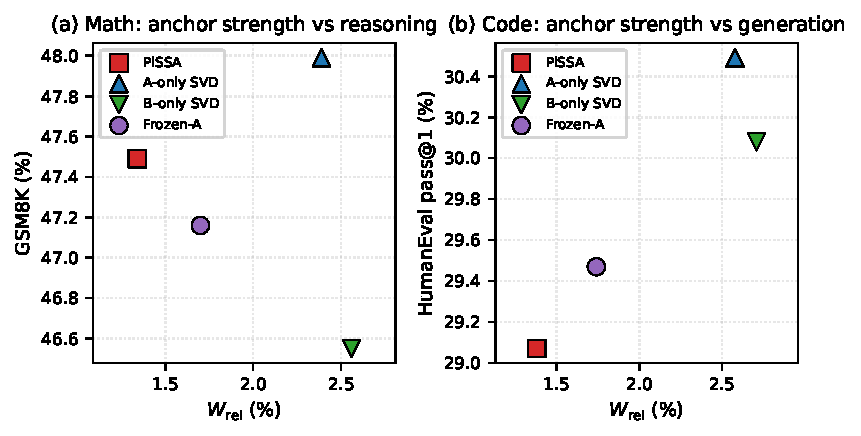
\includegraphics[width=\columnwidth]{figures/w_rel_correlation.pdf}
\caption{$W_{\text{rel}}$과 태스크 성능의 상관관계. PiSSA는 over-anchored 영역(낮은 $W_{\text{rel}}$)에 위치하며, 한쪽 anchor 전략(A/B-only SVD)은 더 큰 $W_{\text{rel}}$로 이동하면서 생성 성능이 향상된다. Frozen-A는 절반 용량으로 PiSSA와 A-only SVD의 중간에 위치하는 최소 실용 어댑터이다.}
\label{fig:w_rel}
\end{figure}

\textbf{(a) PiSSA는 over-anchored 상태이다.} PiSSA의 $W_{\text{rel}}$은 1.34\%로 A-only SVD(2.39\%) 대비 56\% 수준이다. 이는 $A,B$ 모두 SVD anchor에 묶여 학습이 표현할 수 있는 $\Delta W$의 범위가 초깃값 주변으로 제한되기 때문이며, anchor 자체가 해롭다기보다 양쪽 모두 anchor일 때 freedom 쪽이 확보할 수 있는 자유 공간이 사라지는 것이 본질적 원인이다. 그림 1(b)에서 PiSSA가 HumanEval에서 가장 낮은 위치에 있는 것은 다양한 생성이 요구되는 태스크에서 표현 범위 제한의 비용을 보여준다.

\textbf{(b) 한쪽 anchor + 한쪽 freedom의 효과.} A-only / B-only SVD는 한쪽이 SVD anchor로 $W$의 구조적 사전정보를 제공하는 동시에 다른 한쪽이 무작위에서 자유롭게 학습되어 $W_{\text{rel}}$이 PiSSA의 약 1.8--1.9배에 달한다. 이 추가 용량이 두 태스크 모두에서 PiSSA를 능가하는 결과로 이어진다 (그림 1).

\textbf{(c) Frozen-A의 최소 구현.} Frozen-A는 한쪽($A$)을 강하게 SVD로 고정(anchor)했음에도 나머지 한쪽($B$)을 0으로 비워둠(freedom)으로써 PiSSA보다 큰 $W_{\text{rel}}$(1.70\% vs 1.34\%)을 확보할 수 있었다. 이는 한쪽만 닻을 내리는 것이 양쪽을 모두 묶어버리는 것보다 신규 태스크 학습에 필요한 \textit{유연성}을 확보하는 데 유리함을 보여준다. 또한 Frozen-A의 $\text{rel}(B)=0.019$가 A-only SVD의 $\text{rel}(B)=0.018$과 거의 동일하다는 점은 $A$를 학습하지 않아도 $B$ freedom이 동등한 수준의 갱신을 만들어낼 수 있다는 직접 증거이며, 이는 GSM8K 성능 47.16 대 47.99($-0.83$\%p)의 작은 차이로 검증된다.

\textbf{(d) LoRA-FA의 잘못된 anchor 진단.} LoRA-FA는 $A$를 무작위 초기화 후 동결한다는 점에서 Frozen-A와 형식적으로 동일하나, anchor의 방향이 무작위라는 결정적 차이가 있다. GSM8K 33.31\% 대 Frozen-A 47.16\% ($-13.85$\%p), HumanEval 25.41\% 대 29.47\% ($-4.06$\%p)의 압도적 격차는 anchor의 \textit{SVD 방향}이 anchor의 \textit{동결 여부}보다 본질적임을 보여준다. 즉 ``$A$를 동결하는 것''이 효과적인 PEFT 전략이 아니라, ``$W$의 SVD 방향에 anchor한 채 동결하는 것''이 효과적이다. 이는 LoRA-FA 계열의 무작위 동결 전략(VeRA[4] 포함)이 본질적 한계를 가진다.

\subsection*{4.4 추가 분석}

\textbf{Frozen-A의 최고 시드 분석.} 다중 시드에서 Frozen-A의 최고 시드는 GSM8K 48.45\%, HumanEval 29.88\%로 PiSSA의 최고 (각 47.61\%, 29.27\%)을 두 태스크 모두에서 능가한다. 이는 Frozen-A가 좁은 최적화 특성상 시드 분산이 크지만(GSM8K 표준편차 1.62 대 PiSSA 0.12), 적절한 시드에서는 PiSSA의 잠재력을 넘는 표현력을 갖고 있음을 보인다. 추가 검증을 위해 Frozen-A를 5개 시드로 확장한 결과(시드$\in$\{1, 42, 123, 777, 999\}) GSM8K 46.96 $\pm$ 1.18로 3개 시드 결과(47.16 $\pm$ 1.62)와 일관된 분포를 확인하였다.

\textbf{효율성 측면의 의의.} Frozen-A는 학습 파라미터를 24.31M에서 12.39M로 49\% 감소시키며, AdamW의 1차/2차 모멘텀 상태(파라미터당 2배)까지 고려하면 옵티마이저 메모리 절감 효과는 더 크다. PiSSA와 동등한 성능을 절반 용량으로 달성한다는 점에서 Anchor-Freedom 프레임워크의 효율성-성능 Pareto 경계 위에 위치한다.

\section*{5. 결 론}

본 연구는 LoRA의 두 행렬이 anchor와 freedom으로 분업되어야 한다는 프레임워크를 제안하고, $W_{\text{rel}}$ 지표로 6가지 초기화 전략을 다중 시드로 정량 비교하였다. PiSSA의 over-anchoring과 LoRA-FA의 잘못된 anchor가 정량적으로 진단되며, 한쪽 anchor + 한쪽 freedom 전략(A/B-only SVD, Frozen-A)이 PiSSA를 능가함을 보였다. 프레임워크의 최소 구현인 Frozen-A는 학습 파라미터를 49\% 감소시키면서도 표준 LoRA 대비 GSM8K $+3.54$\%p, HumanEval $+1.62$\%p 향상을 달성하며 PiSSA와 동등한 성능을 절반 용량으로 확보한다.

향후 연구로는 (1) 더 큰 모델(7B/13B) 및 다양한 태스크에서의 프레임워크 검증, (2) Anchor의 SVD 방향이 왜 무작위 방향보다 본질적으로 우수한지에 대한 이론적 분석, (3) Anchor-Freedom 비대칭성을 이용한 태스크 산술 가능성을 계획한다.

% =========================================================
% 참고문헌
% =========================================================
\section*{참고문헌}

\begin{small}
\noindent
[1] E. J. Hu et al., ``LoRA: Low-Rank Adaptation of Large Language Models,'' \textit{Proc. ICLR}, 2022.

\noindent
[2] F. Meng, Z. Wang, M. Zhang, ``PiSSA: Principal Singular Values and Singular Vectors Adaptation of Large Language Models,'' \textit{Proc. NeurIPS}, 2024.

\noindent
[3] L. Zhang, L. Zhang, S. Shi, X. Chu, B. Li, ``LoRA-FA: Memory-efficient Low-rank Adaptation for Large Language Models Fine-tuning,'' \textit{arXiv:2308.03303}, 2023.

\noindent
[4] D. J. Kopiczko, T. Blankevoort, Y. M. Asano, ``VeRA: Vector-based Random Matrix Adaptation,'' \textit{Proc. ICLR}, 2024.

\noindent
[5] S.-Y. Liu et al., ``DoRA: Weight-Decomposed Low-Rank Adaptation,'' \textit{Proc. ICML}, 2024.

\noindent
[6] J. Zhang et al., ``LoRI: Reducing Cross-Task Interference in Multi-Task Low-Rank Adaptation,'' \textit{arXiv preprint}, 2025.

\noindent
[7] Meta AI, ``Llama 3.2: Lightweight Models for Edge Devices,'' \url{https://ai.meta.com/blog/llama-3-2}, 2024.

\noindent
[8] K. Cobbe et al., ``Training Verifiers to Solve Math Word Problems,'' \textit{arXiv:2110.14168}, 2021.

\noindent
[9] S. Chaudhary, ``Code Alpaca: An Instruction-following LLaMA Model for Code Generation,'' \url{https://github.com/sahil280114/codealpaca}, 2023.

\noindent
[10] M. Chen et al., ``Evaluating Large Language Models Trained on Code,'' \textit{arXiv:2107.03374}, 2021.
\end{small}

\end{multicols}

\end{document}
